\documentclass[a4paper]{article}
\usepackage{tikz}
\usetikzlibrary{positioning}
\usepackage{subfig}
\usepackage{geometry}
 \geometry{
 a4paper,
 total={170mm,257mm},
 left=0mm,
 top=20mm,
 }

 
\begin{document}
\pagenumbering{gobble}

\begin{figure}[h!]
\centering
\tikz[remember
picture]{\node(1BL){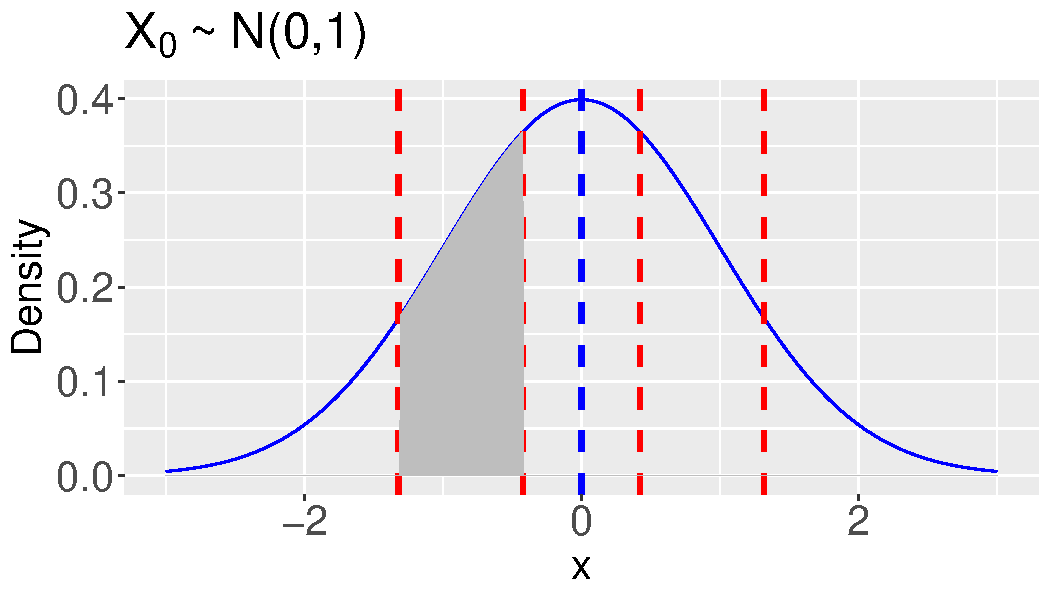
\includegraphics[width=8cm]{../data/X_0.pdf}};}%
\hspace*{3cm}%
\tikz[remember picture]{\node(1BR){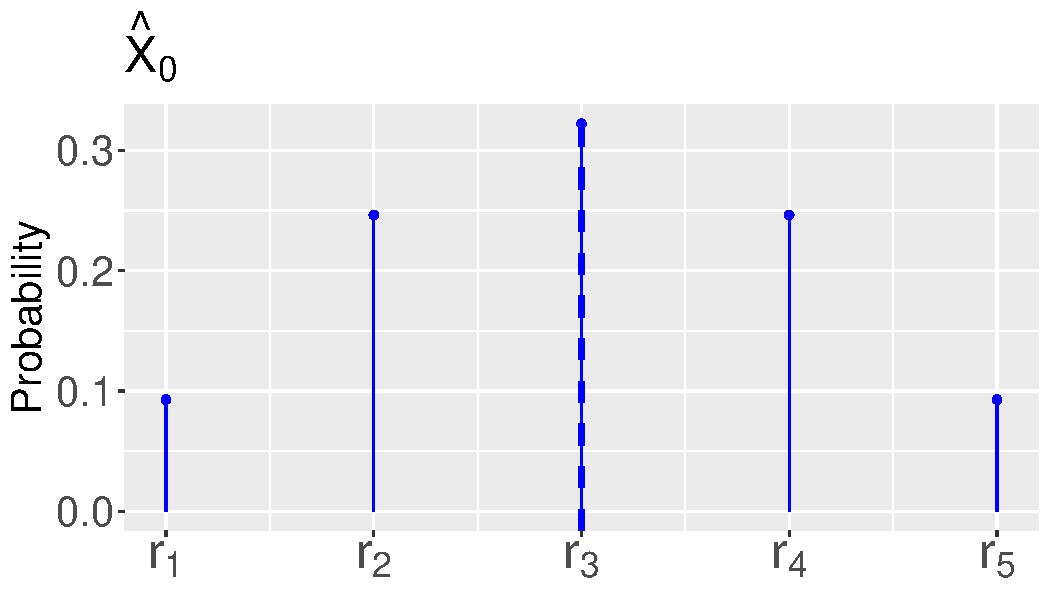
\includegraphics[width=8cm]{../data/X_0_hat.pdf}};}
\end{figure}

\begin{figure}[h!]
\centering
\tikz[remember
picture]{\node(2BL){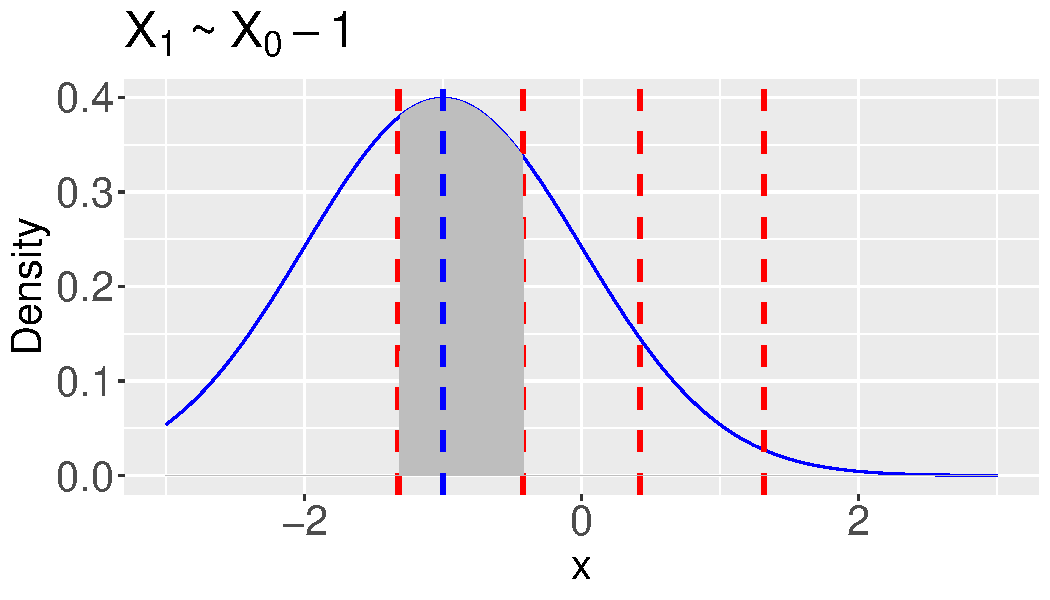
\includegraphics[width=8cm]{../data/X_1.pdf}};}%
\hspace*{3cm}%
\tikz[remember picture]{\node(2BR){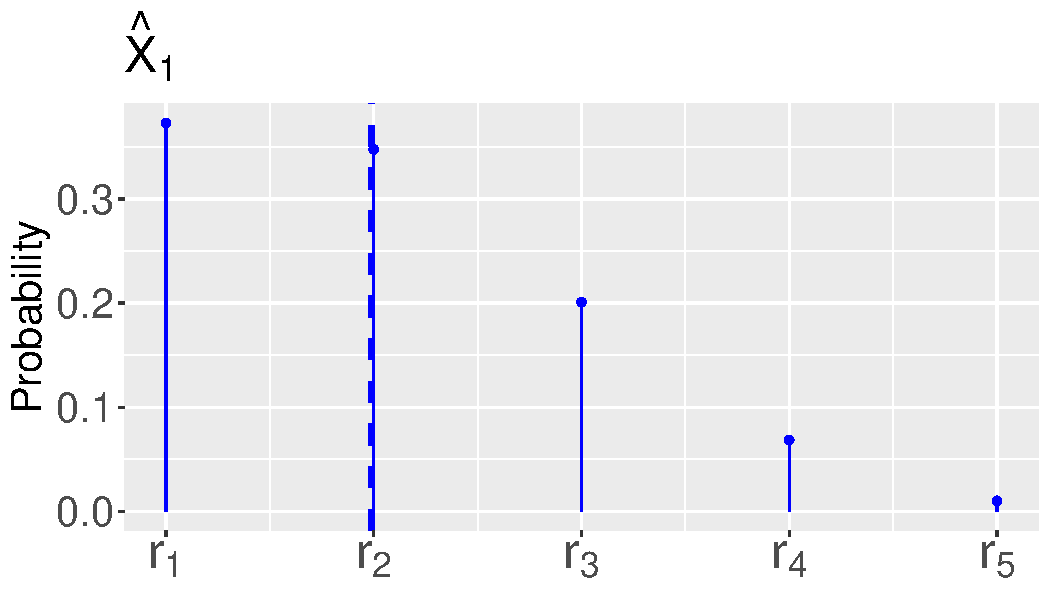
\includegraphics[width=8cm]{../data/X_1_hat.pdf}};}
\end{figure}

\begin{figure}[h!]
\centering
\tikz[remember
picture]{\node(3BL){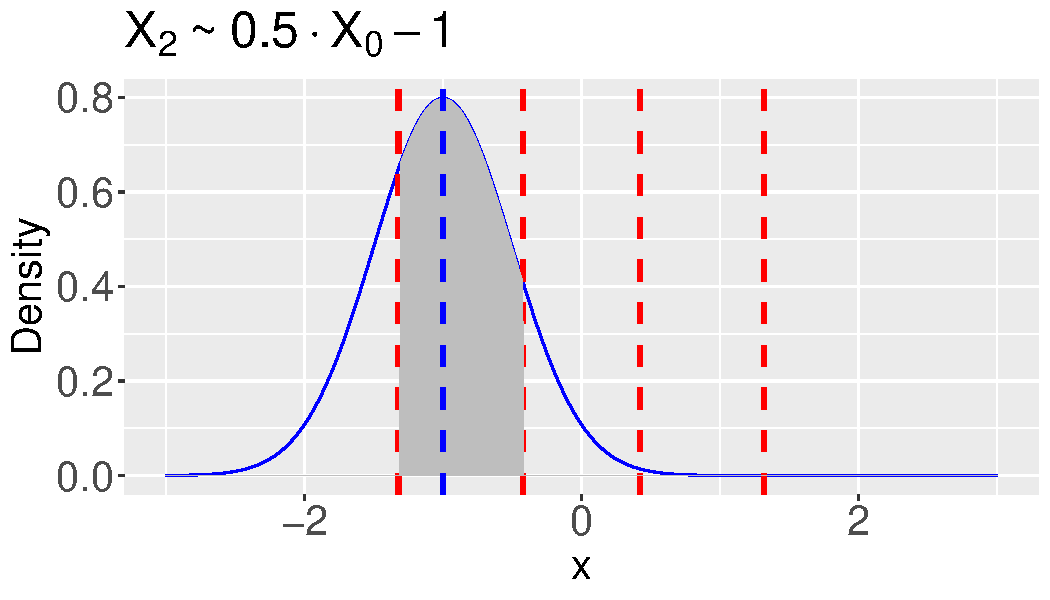
\includegraphics[width=8cm]{../data/X_2.pdf}};}%
\hspace*{3cm}%
\tikz[remember picture]{\node(3BR){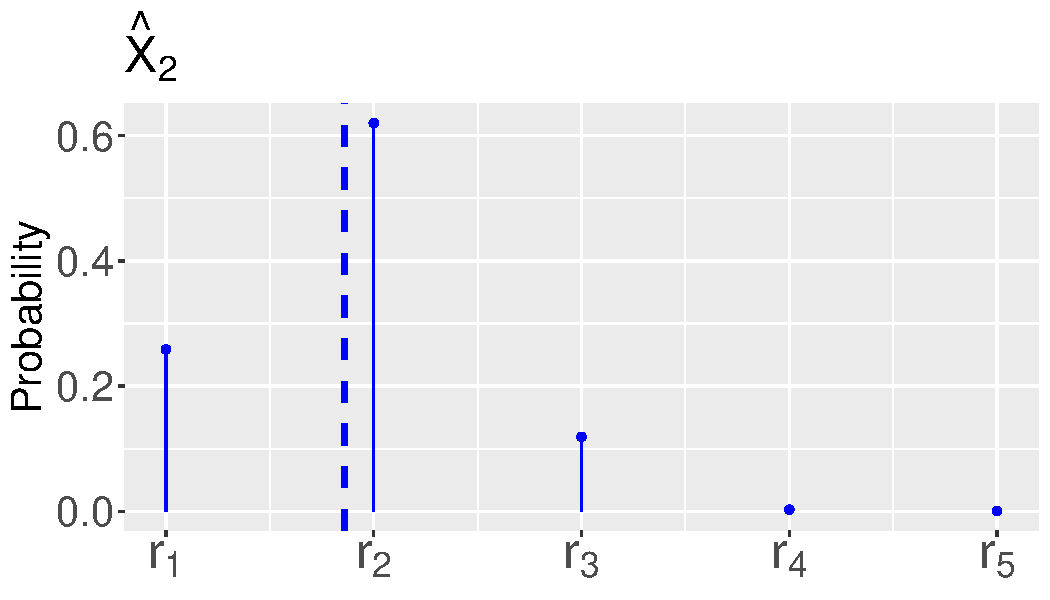
\includegraphics[width=8cm]{../data/X_2_hat.pdf}};}
\end{figure}

\tikz[overlay,remember picture]{\draw[-latex] 
(1BL.east) -- (1BL-|1BR.west)
node[midway,below,text width=0.8cm]{$\mathcal{D}, \mathcal{R}$};}

\tikz[overlay,remember picture]{\draw[-latex] 
(1BL-|1BR.west) -- (1BL)
node[midway,below,text width=0.8cm]{$ $};}


\tikz[overlay,remember picture]{\draw[-latex] 
(2BL.east) -- (2BL-|2BR.west)
node[midway,below,text width=0.8cm]{$\mathcal{D}, \mathcal{R}$};}

\tikz[overlay,remember picture]{\draw[-latex] 
(2BL-|2BR.west) -- (2BL)
node[midway,below,text width=0.8cm]{$ $};}


\tikz[overlay,remember picture]{\draw[-latex] 
(3BL.east) -- (3BL-|3BR.west)
node[midway,below,text width=0.8cm]{$\mathcal{D}, \mathcal{R}$};}

\tikz[overlay,remember picture]{\draw[-latex] 
(3BL-|3BR.west) -- (3BL)
node[midway,below,text width=0.8cm]{$ $};}


\end{document}